\documentclass[tikz,border=4mm]{standalone}
\usepackage{tikz}
\usetikzlibrary{shapes.geometric, arrows}

\tikzstyle{startstop} = [rectangle, rounded corners, 
text width=3cm, 
text height=1cm,
text centered, 
draw=black, 
fill=red!30]

\tikzstyle{io} = [trapezium, 
trapezium stretches=true, % A later addition
trapezium left angle=70, 
trapezium right angle=110, 
text width=3cm, 
text height=1cm,  text centered, 
draw=black, fill=blue!30]

\tikzstyle{process} = [rectangle, 
text width=3cm, 
text height=1cm, 
text centered, 
text width=3cm, 
draw=black, 
fill=orange!30]

\tikzstyle{decision} = [diamond, 
text width=3cm, 
text height=1cm, 
text centered, 
draw=black, 
fill=green!30]
\tikzstyle{arrow} = [thick,->,>=stealth]
\begin{document}
	
	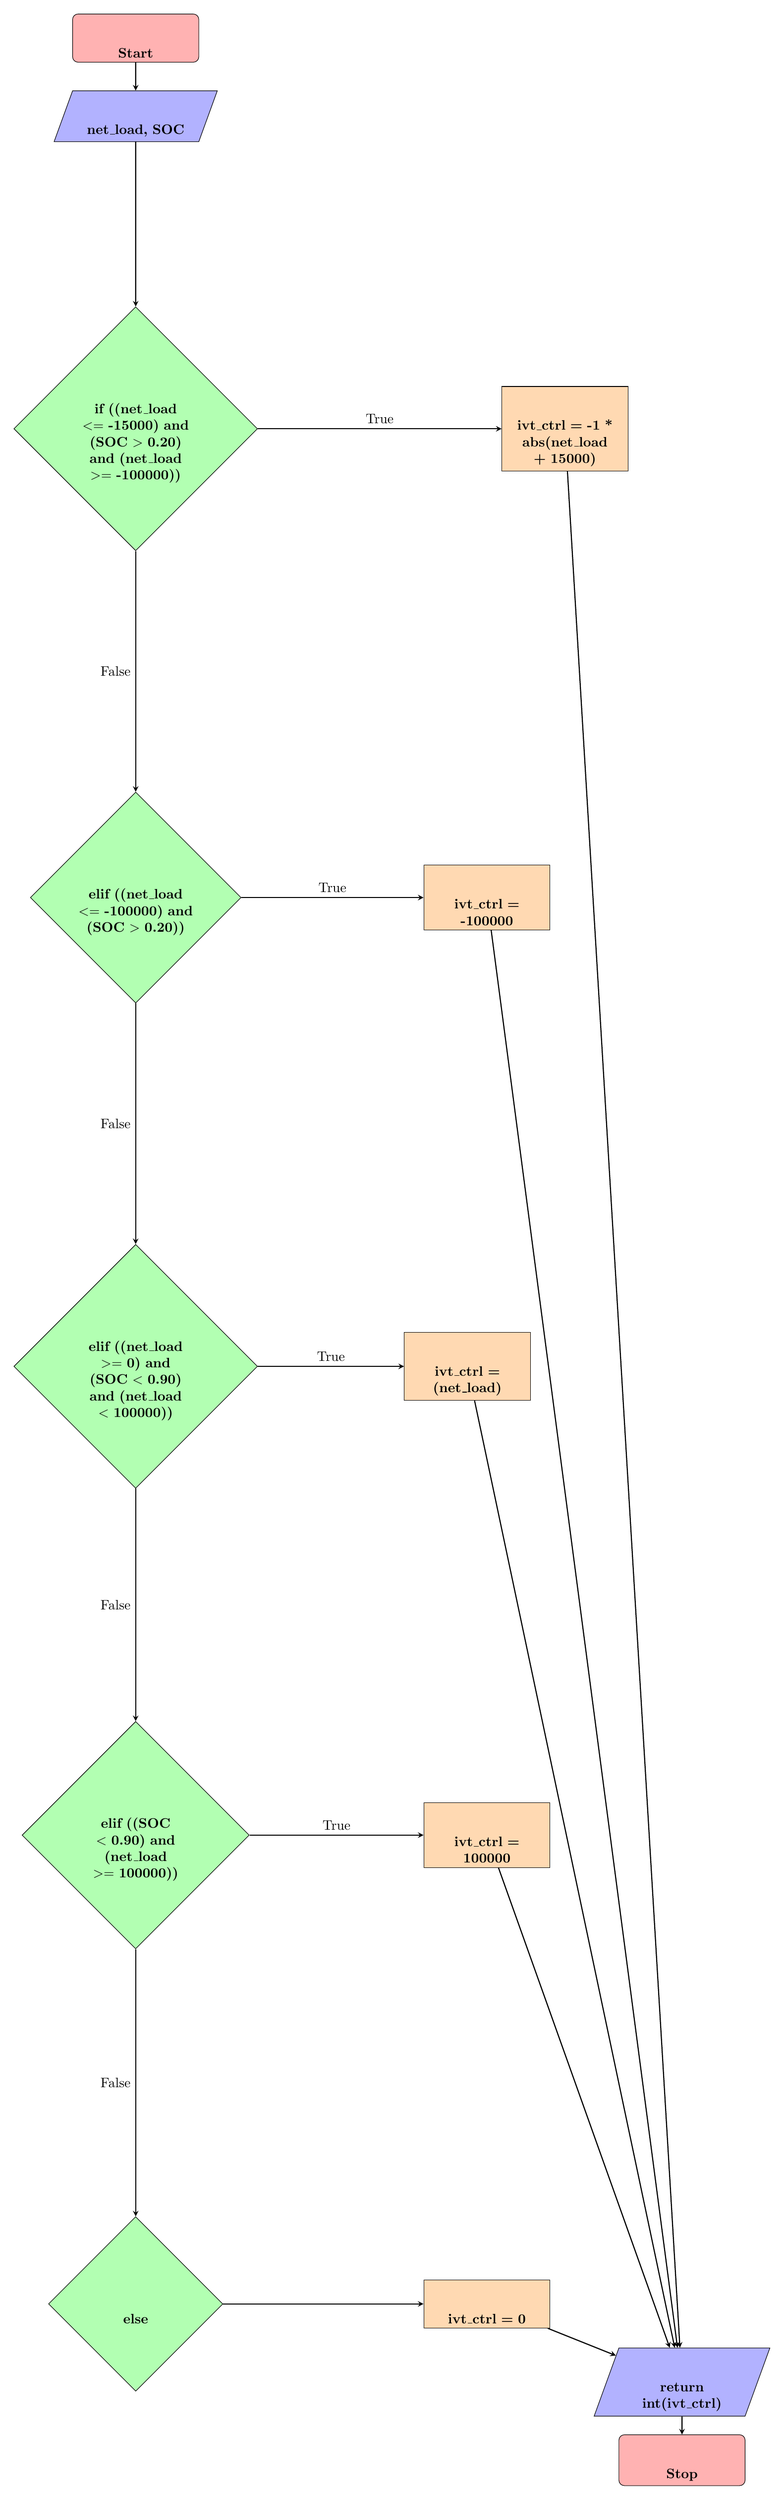
\begin{tikzpicture}[node distance=2cm]
		
		\node (start) [startstop] {\textbf {Start}};
		\node (in1) [io, below of=start] {\textbf {net\_load, SOC}};
	%	\node (pro1) [process, below of=in1] {Process 1};
		
		
%		\node (pro2a) [process, below of=dec1, yshift=-0.5cm] {Process 2a
%			text text text text
%			text text text 
%			text text text};
		\node (dec1) [decision, below of=in1, yshift=-6cm] {\textbf {if ((net\_load $<=$ -15000) and (SOC $>$ 0.20) and (net\_load $>=$ -100000))}};
		\node (dec2) [decision , below of=dec1, yshift= -10cm] {\textbf {elif ((net\_load $<=$ -100000) and (SOC $>$ 0.20))}};
		\node (dec3) [decision , below of=dec2, yshift= -10cm] {\textbf {elif ((net\_load $>=$ 0) and (SOC $<$ 0.90) and (net\_load $<$ 100000))}};
		\node (dec4) [decision , below of=dec3, yshift= -10cm] {\textbf {elif ((SOC $<$ 0.90) and (net\_load $>=$ 100000))}};
		\node (dec5) [decision , below of=dec4, yshift= -10cm] {\textbf {else}};
		
		\node (pro1) [process, right of=dec1, xshift=  9 cm] {\textbf {ivt\_ctrl = -1 * abs(net\_load + 15000)}};
		\node (pro2) [process, right of=dec2, xshift=  7 cm] {\textbf {ivt\_ctrl = -100000}};
		\node (pro3) [process, right of=dec3, xshift=  6.5 cm] {\textbf {ivt\_ctrl = (net\_load)}};
		\node (pro4) [process, right of=dec4, xshift=  7 cm] {\textbf {ivt\_ctrl = 100000}};
		\node (pro5) [process, right of=dec5, xshift=  7 cm] {\textbf {ivt\_ctrl = 0}};
		\node(out1)[io, below of= pro5, xshift =  5 cm] {\textbf {return int(ivt\_ctrl)}};
		\node (stop) [startstop, below of=out1] {\textbf {Stop}};
%		
		\draw [arrow] (start) -- (in1);
		\draw [arrow] (in1) -- (dec1);
		\draw [arrow] (dec1) -- node[anchor=south] {True} (pro1);
		\draw [arrow] (dec1) -- node[anchor=east] {False} (dec2);
		\draw [arrow] (dec2) -- node[anchor=south] {True} (pro2);
		\draw [arrow] (dec2) -- node[anchor=east] {False} (dec3);
		\draw [arrow] (dec3) -- node[anchor=south] {True} (pro3);
		\draw [arrow] (dec3) -- node[anchor=east] {False} (dec4);
		\draw [arrow] (dec4) -- node[anchor=south] {True} (pro4);
		\draw [arrow] (dec4) -- node[anchor=east] {False} (dec5);
		\draw [arrow] (dec5) -- (pro5);
		
		\draw[arrow] (pro1) --  (out1);
		\draw[arrow] (pro2) -- (out1);
		\draw[arrow] (pro3) -- (out1);
		\draw[arrow] (pro4) -- (out1);
		\draw[arrow] (pro5) -- (out1);
		
		\draw[arrow] (out1) -- (stop);
		
%		\draw [arrow] (pro2b) |- (pro1);
%		\draw [arrow] (pro2a) -- (out1);
%		\draw [arrow] (out1) -- (stop);
		
	\end{tikzpicture}
\end{document}